% \documentclass[12pt, a4paper, twoside , openright ]{report}
\documentclass[12pt, a4paper, openright ]{report}
% Encoding and Languages
\usepackage[utf8]{inputenc}
\usepackage[portuguese, english]{babel}

% Font
\usepackage[T1]{fontenc}
% \usepackage{blindtext} % Lorem ipsum...
\usepackage{listings} % Useful for Code blocks
\usepackage{hyperref} % URL


% Identation Setups
\usepackage{indentfirst} % Indentation of First Word in Paragraph (Only required in some cases(?))
    \setlength{\parindent}{16pt}
    \setlength{\parskip}{7pt}
    \newcommand{\hsp}{\hspace{10pt}}

% Redefinition of \section command
%\usepackage[section]{placeins}
% \usepackage{placeins}

% Headers & Footers
\usepackage{fancyhdr}
    \setlength{\headheight}{14.5pt}
    \renewcommand{\headrulewidth}{2pt}
    \renewcommand{\footrulewidth}{1pt}

% Pictures
\usepackage{graphicx, float}
% Tables
\usepackage{multirow, makecell}

% Math Packages
\usepackage{amsmath, amssymb}

% Color Setups
\usepackage{color, xcolor}
    % URL
    \hypersetup{ urlcolor=cyan, }
    % Custom Colors
    \definecolor{lightBlue}{RGB}{54, 95, 145}
    \definecolor{darkBlue}{RGB}{23, 54, 145}
\usepackage{xcolor}

% Sectioning Setup
\usepackage{titlesec}
    % Chapter
\titleformat{\chapter}[hang]{\Huge\bfseries}{}{0pt}{\Huge\bfseries\color{darkBlue}}
\titlespacing{\chapter}{0pt}{-50pt}{20pt} % {command}{left}{before sep} {after sep}[right] default = {0pt}{50pt}{40pt}
    % Section
\titleformat{\section}[hang]{\Large\bfseries}{}{20pt}{\Large\bfseries\color{lightBlue}}
    % SubSection
\titleformat{\subsection}[hang]{\large\bfseries}{}{40pt}{\large\bfseries\color{lightBlue}}

% Headers 
% \pagestyle{fancy}
% \fancyhf{}
% \fancyhead[LE,RO]{Pesquisa do Melhor Horário}
% \fancyfoot[CE,CO]{\leftmark}
% \fancyfoot[LE,RO]{\thepage}

\title{
    \begin{figure}[t]
        \centering
        \includegraphics[scale=0.5]{images/est-banner.png}
    \end{figure}
    
    \large{
            {Licenciatura em Engenharia de Sistemas Informáticos}
        }\\
    \bigskip
	\small{
    	    {No âmbito da UC de Sistemas Embebidos em Tempo Real}
    }\\
    \vfill
    \textbf{
	    \Huge{
	        \textcolor{lightBlue}{\fontsize{48pt}{48pt}{\textit{Home Automation}}}
        }\\
    % 	\large{
    %     	    \textcolor{lightBlue}{}
	   % }\\
        }
    \vfill
	}
\author{André Cardoso \& Leonel Fernandes\\18848 \& 18850}
\date{Barcelos, \selectlanguage{portuguese}\today}

\begin{document}
    \maketitle
    \tableofcontents
    
    \chapter{Contextualização}

Em contexto da Unidade Curricular de Integração de Sistemas Informáticos é proposto encontrar e desenvolver um problema a resolver através do processo de ETL.

O problema em questão deve incorporar processos como, por exemplo: 
\begin{itemize}
    \item Auditorias:
    \begin{itemize}
        \item Dados, Processos, Segurança, etc.
    \end{itemize}
    \item Migração e Reorganização de Dados
    \item Análise e Processamento de Dados (Datamining, etc.)
    \item Recomendações e Previsões sobre Estados com Processamento Recorrente a Big Data
\end{itemize}

\vfill
\small{\textbf{Palavras-chave - ETL} (Extract Transform Load)}
    \chapter*{Introdução}
\addcontentsline{toc}{chapter}{Introdução}

A execução do trabalho prático proposto requer a utilização da plataforma Arduino. Foram utilizados, assim como diversos outros componentes compatíveis com a plataforma, de forma a resolver os 4 sistemas e as variadas funções adicionais requeridas.

Para o Sistema de controlo de iluminação interior, o Arduino deverá ser capaz de analisar os valores lidos de um fotorresistor, para assim alterar a intensidade de um LED.

Para o Sistema de controlo de Climatização, o Arduino deverá ser capaz de analisar os valores lidos de um sensor de temperatura e, através da utilização de um display LCD, apresentá-los de forma legível.

Para o Sistema de Acesso ao Estacionamento, o Arduino deverá ser capaz de analisar o input de um utilizador através de um comando de infravermelhos e assim alterar o posicionamento de um motor Servo, sendo que também deverá ser possível suspender o movimento do mesmo.

Para o Sistema de Segurança, o Arduino deverá ser capaz de analisar o input de um sensor de movimento e de seguida acionar um alarme sonoro.

Será ainda necessário, devido às restrições em termos de Hardware, a junção de sistemas por pares para execução em simultâneo das suas funções.

Todos estes sistemas deverão ter em conta as funções adicionais de necessária implementação em pelo menos um dos sistemas. 

    
    \chapter{Análise de Requisitos}

\section{Requisitos Não Funcionais}
Para este projeto verificamos que os Requisitos Não Funcionais se aplicam a todos os sistemas desenvolvidos, sendo eles:
\begin{itemize}
    \item Processamento em Tempo Real
    \item Consumo energético inferior a 5 Watts
\end{itemize}

\section{Requisitos Funcionais}
\subsection{Sistema A}
\begin{itemize}
    \item Deteção da Intensidade de Luz Solar
    \item Regulação da Intensidade de Luz Artifical\footnote{LED} em função da Intensidade da Luz Solar
\end{itemize}

\subsection{Sistema B}
\begin{itemize}
    \item Deteção da Temperatura Ambiente
    \item Regulação da Temperatura Ambiente
    \begin{itemize}
        \item Através de Ventilação\footnote{Ventoínha}
        \item Em função da Temperatura Ambiente
    \end{itemize}
    \item Enunciar o Estado da Ventilação
    \begin{itemize}
        \item LED de cor Verde - Temperatura `Estável'
        \item LED de cor Vermelha - Arrefecimento Ambiente
    \end{itemize}\newpage
    \item Apresentação por LCD\footnote{Liquid Crystal Display} de:
    \begin{itemize}
        \item Estado da Ventoínha (ON/OFF)
        \item Última Temperatura Lida
    \end{itemize}
    \item Controlo de Luminosidade do LCD
\end{itemize}

% \newpage

\subsection{Sistema C}
\begin{itemize}
    \item Controlo Remoto de uma Barra de Acesso a Parque de Estacionamento
    \begin{itemize}
        \item Abertura
        \item Fecho
    \end{itemize}
    \item Capacidade de Suspensão da Atividade atual da Barra 
    \item Deteção de Movimento - Sensor Ultrassônico
\end{itemize}

\subsection{Sistema D}
\begin{itemize}
    \item Deteção de Movimento Intrusivo
    \item Sinalização de Intrusões
    \begin{itemize}
        \item Sonora - Alarme
        \item Visual - LED Intermitente
    \end{itemize}
    \item Capacidade de desarmar o Alarme
\end{itemize}
    \chapter{Especificação do Sistema}

\section{Hardware - Arduino Uno R3}
\begin{figure}[H]
    \centering
    \includegraphics[scale=0.15]{images/Arduino_Board.jpg}
    \selectlanguage{portuguese}\caption{Arduino Uno R3}
\end{figure}
O design da PCB do Arduino Uno utiliza componentes SMD\footnote{Surface Mount Device}.

O micro-controlador inserido nesta placa é o \textbf{ATmega328} - MCU\footnote{Micro Controller Unit} da família AVR\footnote{Alf and Vegard's RISC} e Arquitetura Harvard (armazena o programa e as variáveis em unidades diferentes.). É um dispositivo de 8-bits, isto é, a sua arquitetura é capaz de gerir 8 sinais em paralelo.

Este chip tem 3 tipos de memória:
\begin{itemize}
    \item \textbf{Flash}: 32kB. Utilizada para armazenar o código compilado da aplicação, dado ser memória \textbf{Não Volátil}.
    \item \textbf{SRAM}: 2kB. Armazenamento de variáveis. \textbf{Volátil}.
    \item \textbf{EEPROM}: 1kB. Armazenamento de dados, que necessitam persistência. \textbf{Não Volátil}.
\end{itemize}

Para armazenamento do código compilado, dado que a MCU não é capaz de comunicar diretamente por USB, precisa de uma `ponte' que converta os sinais do host USB para a interface UART\footnote{Universal Asynchronous Receiver-Transmiter} - o \textbf{ATmega16U2}.

\begin{figure}[H]
    \centering
    \includegraphics[scale=0.8, angle=-90]{images/atmega16u2.png}
    \selectlanguage{portuguese}\caption{ATmega16U2}
\end{figure}

\section{Software - C/C++}

Para facilidade de uso pelos consumidores o \textit{chipset} (ATmega328) é previamente programado com um \textit{\textbf{bootloader}}. Este é basicamente o controlador do processo de `arranque' da placa Arduino.

Dado que o código é desenvolvido numa arquitetura diferente da arquitetura destino (x86\_x64 para Arm), o código é compilado em \textit{cross-compiling} e denominado de \textit{\textbf{firmware}}. É carregado via USB como discutido anteriormente e apenas uma vez, dada a persistência da memória. 
\newpage
Exemplo de \textit{cross-compiling} de programa(em ambiente Linux baseado em Debian/Ubuntu).

\begin{lstlisting}[language=bash]
// Install packages
sudo apt-get install gcc-arm-linux-gnueabi 
g++-arm-linux-gnueabi

// Compile
arm-linux-gnueabi-gcc helloworld.c -o helloworld-arm 
-static
// Run
./helloworld-arm
// Read Architecture
readelf -h helloworld-arm
\end{lstlisting}
    \chapter{Modelo de Conceção}

Para desenvolvimento do projeto em mãos consideramos que o mais lógico seria seguir um modelo de desenvolvimento `Waterfall'.

O modelo Waterfall obedece a seguinte estrutura:
\begin{enumerate}
    \item Requisitos
    \item Arquitetura
    \item Codificação
    \item Teste
    \item Manutenção
\end{enumerate}

Apesar de ser um modelo de conceção pouco utilizado atualmente, dado o nosso caso de uso acreditamos que se enquadra perfeitamente dado que:
\begin{itemize}
    \item Não haverá alteração de Requisitos
    \item O Hardware já está em nossa posse\\ (Sendo a \textbf{necessidade de assunção} deste uma das desvantagens apontadas)
\end{itemize}
    
    % Hardware
    \chapter{Construção do Sistema - Hardware}
    \section{Sistema A – Controlo de Iluminação Interior}


\begin{figure}[H]
    \centering
    \includegraphics[scale=0.6]{images/hardware/sisA_tinkercad.png}
    \selectlanguage{portuguese}\caption{Esquema do Sistema A}
\end{figure}

\begin{figure}[H]
\centering
\setlength{\arrayrulewidth}{0.5mm}
\renewcommand{\arraystretch}{1.5}
\begin{tabular}{|l | c|} 
 \hline
 \multicolumn{1}{|c|}{Componentes} & \multicolumn{1}{|c|}{Quantidade}\\ [0.8ex] 
 \hline
 Fotorresistor & 1x \\ 
 \hline
 Botão & 1x \\
 \hline
 Arduino & 1x \\
 \hline
 Breadboard & 1x\\
 \hline
 LED & 1x\\
 \hline
 Resistência 330 Ohm & 1x\\
 \hline
 Resistência 10k Ohm & 2x  \\
 \hline
\end{tabular}
\selectlanguage{portuguese}\caption{Componentes Utilizados}
\end{figure}

A resistência de 330 Ohm encontra-se ligada ao LED.

As duas resistências de 10k Ohm encontram-se ligadas ao fotorresistor e ao botão.

O Arduino recebe o input do fotorresistor através do pino analógico A1.

O LED está ligado à porta nº 3 que serve como output.

O Arduino recebe o input do botão através da porta nº 2. O Botão serve de interrupt do sistema.

\begin{figure}[H]
    \centering
    \includegraphics[scale=0.05,angle=90]{images/hardware/sisA_IRL.jpg}
    \selectlanguage{portuguese}\caption{Esquema montado do Sistema A}
\end{figure}
    \newpage
\section{Sistema B – Controlo de Climatização}


\begin{figure}[H]
    % \centering
    \includegraphics[scale=0.5]{images/hardware/sisB_tinkercad.png}
    \selectlanguage{portuguese}\caption{Esquema do Sistema}
\end{figure}
% A solução deste sistema exige a utilização de:
\begin{table}[H]
    \centering
    \setlength{\arrayrulewidth}{0.5mm}
    \renewcommand{\arraystretch}{1.5}
    \begin{tabular}{|l|c|}
        \hline
        \multicolumn{1}{|c|}{Componentes} & \multicolumn{1}{|c|}{Quantidade}\\ [0.8ex] 
        \hline
        Arduino & 1x\\
        \hline
        LCD 16x2 & 1x\\
        \hline
        Potenciómetro 10k$\Omega$ & 1x\\
        \hline
        Sensor de Temperatura DHT11 & 1x\\
        \hline
        LED Vermelho & 1x\\
        \hline
        LED Verde & 1x\\
        \hline
        Resistência 220$\Omega$ & 3x\\
        \hline
    \end{tabular}
    \selectlanguage{portuguese}
    \caption{Lista dos Componentes}
\end{table}

O LCD está ligado à placa Arduino do seguinte modo:\\
(Da esquerda para a direita do LCD)
\begin{itemize}
    \item GCC -- GND
    \item VCC -- 5V
    \item V0 -- Pino Analógico do Potenciómetro
    \item RS -- 13
    \item RW -- GND
    \item E -- 12
    \item D0 > D3 -- Desconectados
    \item D4 -- 8
    \item D5 -- 9
    \item D6 -- 10
    \item D7 -- 11
\end{itemize}

O sensor de temperatura, que no esquema físico corresponde ao modelo DHT11, encontra-se ligado à porta digital n$^{o}$ 7.

Os LED's Verde e Vermelho encontram-se ligados às portas analógicas 5 e 4 respetivamente.
    \section{Sistema C – Sistema Acesso ao Estacionamento}

\begin{figure}[H]
    \centering
    \includegraphics[scale=0.4]{images/hardware/sisC_tinkercad.png}    
    \selectlanguage{portuguese}\caption{Esquema do Sistema C}
\end{figure}

\begin{figure}[H]
\centering
\setlength{\arrayrulewidth}{0.5mm}
\renewcommand{\arraystretch}{1.5}
\begin{tabular}{|l | c|} 
 \hline
 \multicolumn{1}{|c|}{Componentes} & \multicolumn{1}{|c|}{Quantidade}\\ [0.8ex] 
 \hline
 Sensor Infravermelhos & 1x \\ 
 \hline
 Motor Servo & 1x \\
 \hline
 Arduino & 1x \\
 \hline
 Breadboard & 1x\\
 \hline
 Comando Infravermelhos & 1x  \\ 
 \hline
\end{tabular}
\selectlanguage{portuguese}\caption{Componentes Utilizados}
\end{figure}


O Sensor infravermelhos encontra-se ligado à porta nº 11 para envio dos dados.

O motor Servo encotra-se ligado à porta nº 8 para ser controlado pelo arduino.



\begin{figure}[H]
    \centering
    \includegraphics[scale=0.05]{images/hardware/sisC_IRL.jpg}
    \selectlanguage{portuguese}\caption{Esquema montado do Sistema A}
\end{figure}
    \newpage\section{Sistema D – Sistema de Segurança}


\begin{figure}[H]
    \centering
    \includegraphics[scale=0.6,angle=-90]{images/hardware/sisD_tinkercad.png}
    \selectlanguage{portuguese}\caption{Esquema do Sistema}
\end{figure}

\begin{table}[H]
    \centering
    \setlength{\arrayrulewidth}{0.5mm}
    \renewcommand{\arraystretch}{1.5}
    \begin{tabular}{|l|c|}
        \hline
        \multicolumn{1}{|c|}{Componentes} & \multicolumn{1}{|c|}{Quantidade}\\ [0.8ex] 
        \hline
        Arduino & 1x\\
        \hline
        LED Vermelho & 1x\\
        \hline
        Alarme Sonoro & 1x\\
        \hline
        Botão & 1x\\
        \hline
        Resistência 220$\Omega$ & 1x\\
        \hline
        Resistência 1k$\Omega$ & 1x\\
        \hline
    \end{tabular}
    \selectlanguage{portuguese}
    \caption{Lista dos Componentes}
\end{table}

O botão encontra-se ligado à porta digital n$^{o}$ 3.

O sensor PIR está ligado à porta digital n$^{o}$2.

O LED Vermelho encontra-se ligado à porta analógica n$^{o}$1.

As portas 2 e 3 apresentam capacidade de Interrupt.
    \newpage\section{Sistema A + C}

\begin{figure}[H]
    \centering
    \includegraphics[scale=0.45]{images/hardware/sisAC_tinkercadUltrassonic.png}
    \selectlanguage{portuguese}\caption{Esquema do Sistema}
\end{figure}

\begin{table}[H]
    \centering
    \setlength{\arrayrulewidth}{0.5mm}
    \renewcommand{\arraystretch}{1.5}
    \begin{tabular}{|l|c|}
        \hline
        \multicolumn{1}{|c|}{Componentes} & \multicolumn{1}{|c|}{Quantidade}\\ [0.8ex] 
        \hline
        Arduino & 1x\\
        \hline
        LED Vermelho & 1x\\
        \hline
        Resistência 330$\Omega$ & 1x\\
        \hline
        Resistência 10k$\Omega$ & 2x\\
        \hline
        Botão & 1x\\
        \hline
        Sensor IR & 1x\\
        \hline
        Comando IR & 1x\\
        \hline
        Sensor Ultrassónico & 1x\\
        \hline
        Fotorresistor & 1x\\
        \hline
        Servomotor & 1x\\
        \hline
        
    \end{tabular}
    \selectlanguage{portuguese}
    \caption{Lista dos Componentes}
\end{table}

\begin{figure}[H]
    \centering
    \includegraphics[scale=0.08]{images/hardware/sisAC_IRL.jpg}
    \selectlanguage{portuguese}\caption{Sistema Montado}
\end{figure}
    \newpage\section{Sistema B + D}

\begin{figure}[H]
    \centering
    \includegraphics[scale=0.6]{images/hardware/sisBD.png}
    \selectlanguage{portuguese}\caption{Esquema do Sistema}
\end{figure}
    
    % Software
    \input{software/070.software}
    \section{Sistema A – Controlo de Iluminação Interior}

O Sistema A tem como objetivo o controlo de um LED através de um fotorresistor. Foi ainda incluído um interrupt que fuciona através de um botão que desabilita o funcionamento do LED. O código elaborado foi o seguinte:

\begin{figure}[H]
    \centering
    \includegraphics[scale=0.5]{images/codigo/sisA_ledvalues.png}
    \selectlanguage{portuguese}\caption{Código para os níveis o LED}
\end{figure}


\begin{itemize}
    \item 1 - O valor do Fotorresistor é lido através da função analogRead no pino onde está ligado o mesmo.
    \item 2,3,4,5 - Para o caso do LED estar compreendido dentro dos valores do "if", o mesmo é acendido com diferentes valores de potência. 
\end{itemize}

\begin{figure}[H]
    \centering
    \includegraphics[scale=0.5]{images/codigo/sisA_interruptsetup.png}
    \selectlanguage{portuguese}\caption{Código para o setup do interrupt}
\end{figure}

\begin{figure}[H]
    \centering
    \includegraphics[scale=0.5]{images/codigo/sisA_interruptfunction.png}
    \selectlanguage{portuguese}\caption{Código para a função do interrupt}
\end{figure}

\begin{itemize}
    \item 1 - O LED é desligado durante o interrupt.
    \item 2 - Enquanto o botão se encontra pressionado, este "while" mantém a função de interrupt a correr.
\end{itemize}

    \section{Sistema B – Controlo de Climatização}

É requisitado que dada uma temperatura, obtida através do sensor DHT, e um intervalo de temperaturas máxima e mínima (25 e 20, respetivamente), o sistema seja capaz de manter uma temperatura ambiente controlada com recurso a uma ventoínha.

Como tal, sempre que a temperatura ultrapassar a temperatura \textbf{máxima}, a ventoínha deve ser acionada até que a temperatura registada seja inferior à temperatura \textbf{mínima}.

\begin{figure}[H]
    \centering
    \includegraphics{images/codigo/sisB_loop.png}
    \selectlanguage{portuguese}\caption{Função loop()}
\end{figure}

Esta função controla o `flow' do Programa. Como se pode verificar, está definido o controlo de temperatura seguido da atualização do LCD. Por fim, um delay para estabilidade das leituras e apresentação do LCD.

\begin{figure}[H]
    \centering
    \includegraphics[scale=0.5]{images/codigo/sisB_temp.png}
    \selectlanguage{portuguese}\caption{Função temp\_control()}
\end{figure}

\begin{enumerate}
  \setcounter{enumi}{-1}
    \item Falha de leitura da temperatura pelo sensor DHT
    \item Definição do estado da ventoínha em função da temperatura observada.
    \begin{itemize}
        \item Transição entre estado \textbf{estável} e \textbf{arrefecimento}
        \item Transição entre estado \textbf{arrefecimento} e \textbf{estável}
    \end{itemize}
    \item Definição do estado do sistema utilizando LEDs em função do estado da ventoínha.
\end{enumerate}

\begin{figure}[H]
    \centering
    \includegraphics[scale=0.5]{images/codigo/sisB_lcd.png}
    \selectlanguage{portuguese}\caption{Função lcd\_update()}
\end{figure}

\begin{enumerate}
    \item Limpeza do ecrã do LCD e consequente reposiçãodo cursor.
    \item Apresentação do estado atual da Ventoínha.
    \item Definição do caracter `$^{o}$'.
    \item Apresentação da última temperatura lida.
\end{enumerate}
    \section{Sistema C – Sistema Acesso ao Estacionamento}


O Sistema C tem como objetivo o controlo de um motor servo através de um comando de infravermelhos. O motor servo servirá como "portão". Deverá ser possível levantar e baixar o portão, assim como suspender o seu movimento. O programa apresenta ainda "multitasking" por "timer", para ser possível ler os valores do comando e alterar a posição do servo simultaneamente. O código elaborado foi o seguinte:


\begin{figure}[H]
    \centering
    \includegraphics[scale=0.6]{images/codigo/sisC_codigosComando.png}
    \selectlanguage{portuguese}\caption{Código para o comando IR}
\end{figure}

\begin{figure}[H]
    \centering
    \includegraphics[scale=0.6]{images/codigo/sisC_definicaoRecetor.png}
    \selectlanguage{portuguese}\caption{Definição do sensor IR}
\end{figure}

\begin{figure}[H]
    \centering
    \includegraphics[scale=0.5]{images/codigo/sisC_remoteFunctionRead.png}
    \selectlanguage{portuguese}\caption{Função de leitura de valor do Sensor IR}
\end{figure}

\begin{itemize}
    \item 1 - Leitura do valor recebido pelo sensor de Infravermelhos.
    \item 2 - Caso o código seja um dos códigos definidos a variável "state" é alterada, esta variável serve para controlar o funcionamento do servo.
\end{itemize}

\begin{figure}[H]
    \centering
    \includegraphics[scale=0.6]{images/codigo/sisC_servofunction.png}
    \selectlanguage{portuguese}\caption{Função para controlo do Servo}
\end{figure}

Esta função serve para alterar a posição do servo em 1 grau por cada iteração do programa, apenas no caso do "state" se encontrar igual a "0" ou "1".


\begin{figure}[H]
    \centering
    \includegraphics[scale=0.6]{images/codigo/sisC_definicaoMultitasking.png}
    \selectlanguage{portuguese}\caption{Definições para multitasking}
\end{figure}

\begin{itemize}
    \item 1 - Definidos os "delays" entre iterações de cada uma das funções.
    \item 2 - As funções para multitasking encontram-se aqui definidas.
\end{itemize}

\begin{figure}[H]
    \centering
    \includegraphics[scale=0.6]{images/codigo/sisC_multitaskingLoop.png}
    \selectlanguage{portuguese}\caption{Loop multitasking}
\end{figure}

\begin{itemize}
    \item 1 - São verficados sempre os milisegundos atuais para execução das funções por timer.
    \item 2 - Execução das funções apenas se se encotrarem no intervalo de tempo correto.
\end{itemize}
    \section{Sistema D – Sistema de Segurança}

É fundamental para o sistema que a cada movimento detetado seja `disparado' um alarme sonoro em conjunto com um LED intermitente. Mais ainda, deve ser possível terminar o alarme com o pressionar de um botão.

Como tal, considerando a importância de cada ação, foi decidida a implementação de ambas em torno do conceito de interrupção do sistema.

\begin{figure}[H]
    \centering
    \includegraphics{images/codigo/sisD_loop.png}
    \caption{Função loop()}
    \label{fig:my_label}
\end{figure}

Podemos verificar que o Programa apenas executa:
\begin{enumerate}
    \item A funcionalidade de alarme, quando o alarme estiver acionado
    \item Suspensão de alarme
\end{enumerate}

As seguintes funções são chamadas por interrupts acionados pelo Sensor PIR e um botão, respetivamente.

\begin{figure}[H]
    \centering
    \includegraphics{images/codigo/sisD_interrupts.png}
    \caption{Funções de Chamadas de Interrupt}
    \label{fig:my_label}
\end{figure}


\begin{enumerate}
    \item \textbf{AlarmOn()} -- Chamada por movimento detetado pelo Sensor.
    \item \textbf{AlarmOff()} -- Chamada por pressão de botão.
\end{enumerate}
    \section{Sistema A + C}


Para junção dos sistemas A e C em termos de código foi apenas utilizado multitasking por timer para poder fazer correr as funções de ambos os sistemas em sincronia. Foi ainda adicionado um sensor ultrassónico para poder fazer a paragem do servomotor.

\begin{figure}[H]
    \centering
    \includegraphics[scale=0.45]{images/codigo/sisACMultitasking.png}
    \selectlanguage{portuguese}\caption{Loop Multitasking}
\end{figure}


\begin{figure}[H]
    \centering
    \includegraphics[scale=0.45]{images/codigo/sisAC_ultra.png}
    \selectlanguage{portuguese}\caption{Função Sensor Ultrassónico}
\end{figure}


    \newpage\section{Sistema B + D}

Para execução dos dois sistemas em tempo real, utilizamos a biblioteca FreeRTOS disponível para Arduino.

\begin{figure}[H]
    \centering
    \includegraphics[scale=0.9]{images/codigo/sisBD_tasks.png}
    \caption{Criação das Tarefas}
    \label{fig:my_label}
\end{figure}

\begin{enumerate}
    \item Tarefa para Alarme Sonoro
    \begin{itemize}
        \item Prioridade -- 2
        \item Handle -- HandleBuzzer
    \end{itemize}
    \item Tarefa para Alarme Visual (LED Intermitente)
    \begin{itemize}
        \item Prioridade -- 2
        \item Handle -- HandleBlink
    \end{itemize}
    \item Tarefa para Alarme Sonoro
    \begin{itemize}
        \item Prioridade -- 0 (Iddle)
        \item Handle -- NULL (Não é necessário)
    \end{itemize}
\end{enumerate}
\newpage
Nesta junção os sistemas mantêm o mesmo funcionamento e como tal o Sistema D continua a fazer uso de Interrupts:

\begin{figure}[H]
    \centering
    \includegraphics[scale=0.9]{images/codigo/sisBD_on.png}
    \caption{Função Interrupção (Deteção Intruso)}
    \label{fig:my_label}
\end{figure}

\begin{enumerate}
    \item Chamada/Notificação da Tarefa TaskBuzzer() (utilizando a `Handle' associada)
    \item Chamada/Notificação da Tarefa TaskBlink() (utilizando a `Handle' associada)
\end{enumerate}

\begin{figure}[H]
    \centering
    \includegraphics{images/codigo/sisBD_off.png}
    \caption{Função Interrupção (Desarme de Alarme)}
    \label{fig:my_label}
\end{figure}

Apesar da disponibilidade da biblioteca FreeRTOS, após alguma pesquisa e experiências, posso afirmar que o Arduino Uno, a placa em utilização, não está preparada a 100\% para lidar com Sistemas Operativos em Tempo Real, um dos problemas que revelou foi a não execução da TaskBuzzer() na situação da TaskBlink() estar descomentada. 
Também verifiquei que não era possível chamar qualquer uma das Tasks se a outra não fosse também criada na inicialização do programa. No entanto, foi possível executar ambas as funções mesmo que não ao mesmo tempo.

Não encontrei resposta para este problema, mesmo após uma pesquisa exaustiva.
\newpage
Assim sendo, foi feito uso da TaskBuzzer() apenas:

\begin{figure}[H]
    \centering
    \includegraphics[scale=0.5]{images/codigo/sisBD_buzzer.png}
    \caption{Caption}
    \label{fig:my_label}
\end{figure}

\begin{enumerate}
    \item Variáveis para Alarme Sonoro e Visual
    \item A tarefa aguarda neste momento por ser chamada
    \item Execução do Alarme
    \item Execução do Desarme
\end{enumerate}
    
    % Teste
    \chapter{Testes}

Gravações dos Sistemas em Funcionamento em Anexo.
    \section{Sistema A – Controlo de Iluminação Interior}

Com um nível de luz entre 0 e 200 o LED encontra-se desligado.


\begin{figure}[H]
    \centering
    \includegraphics[scale=1.1]{images/testes/SisA_SerialMonitor0FF_original.png}
    \includegraphics[scale=0.03]{images/testes/sisA_Off.jpg}
    \selectlanguage{portuguese}\caption{LED desligado no nivel inicial}
\end{figure}


Com um nível de luz entre 200 e 500 o LED encontra-se ligado com um valor de 64.

\begin{figure}[H]
    \centering
    \includegraphics[scale=1.1]{images/testes/sisA_SerialMonitor1_original.png}
    \includegraphics[scale=0.03]{images/testes/sisA_1.jpg}
    \selectlanguage{portuguese}\caption{LED ligado no nivel 1}
\end{figure}

Com um nível de luz entre 500 e 800 o LED encontra-se ligado com um valor de 128.

\begin{figure}[H]
    \centering
    \includegraphics[scale=1.1]{images/testes/sisA_SerialMonitor2_original.png}
    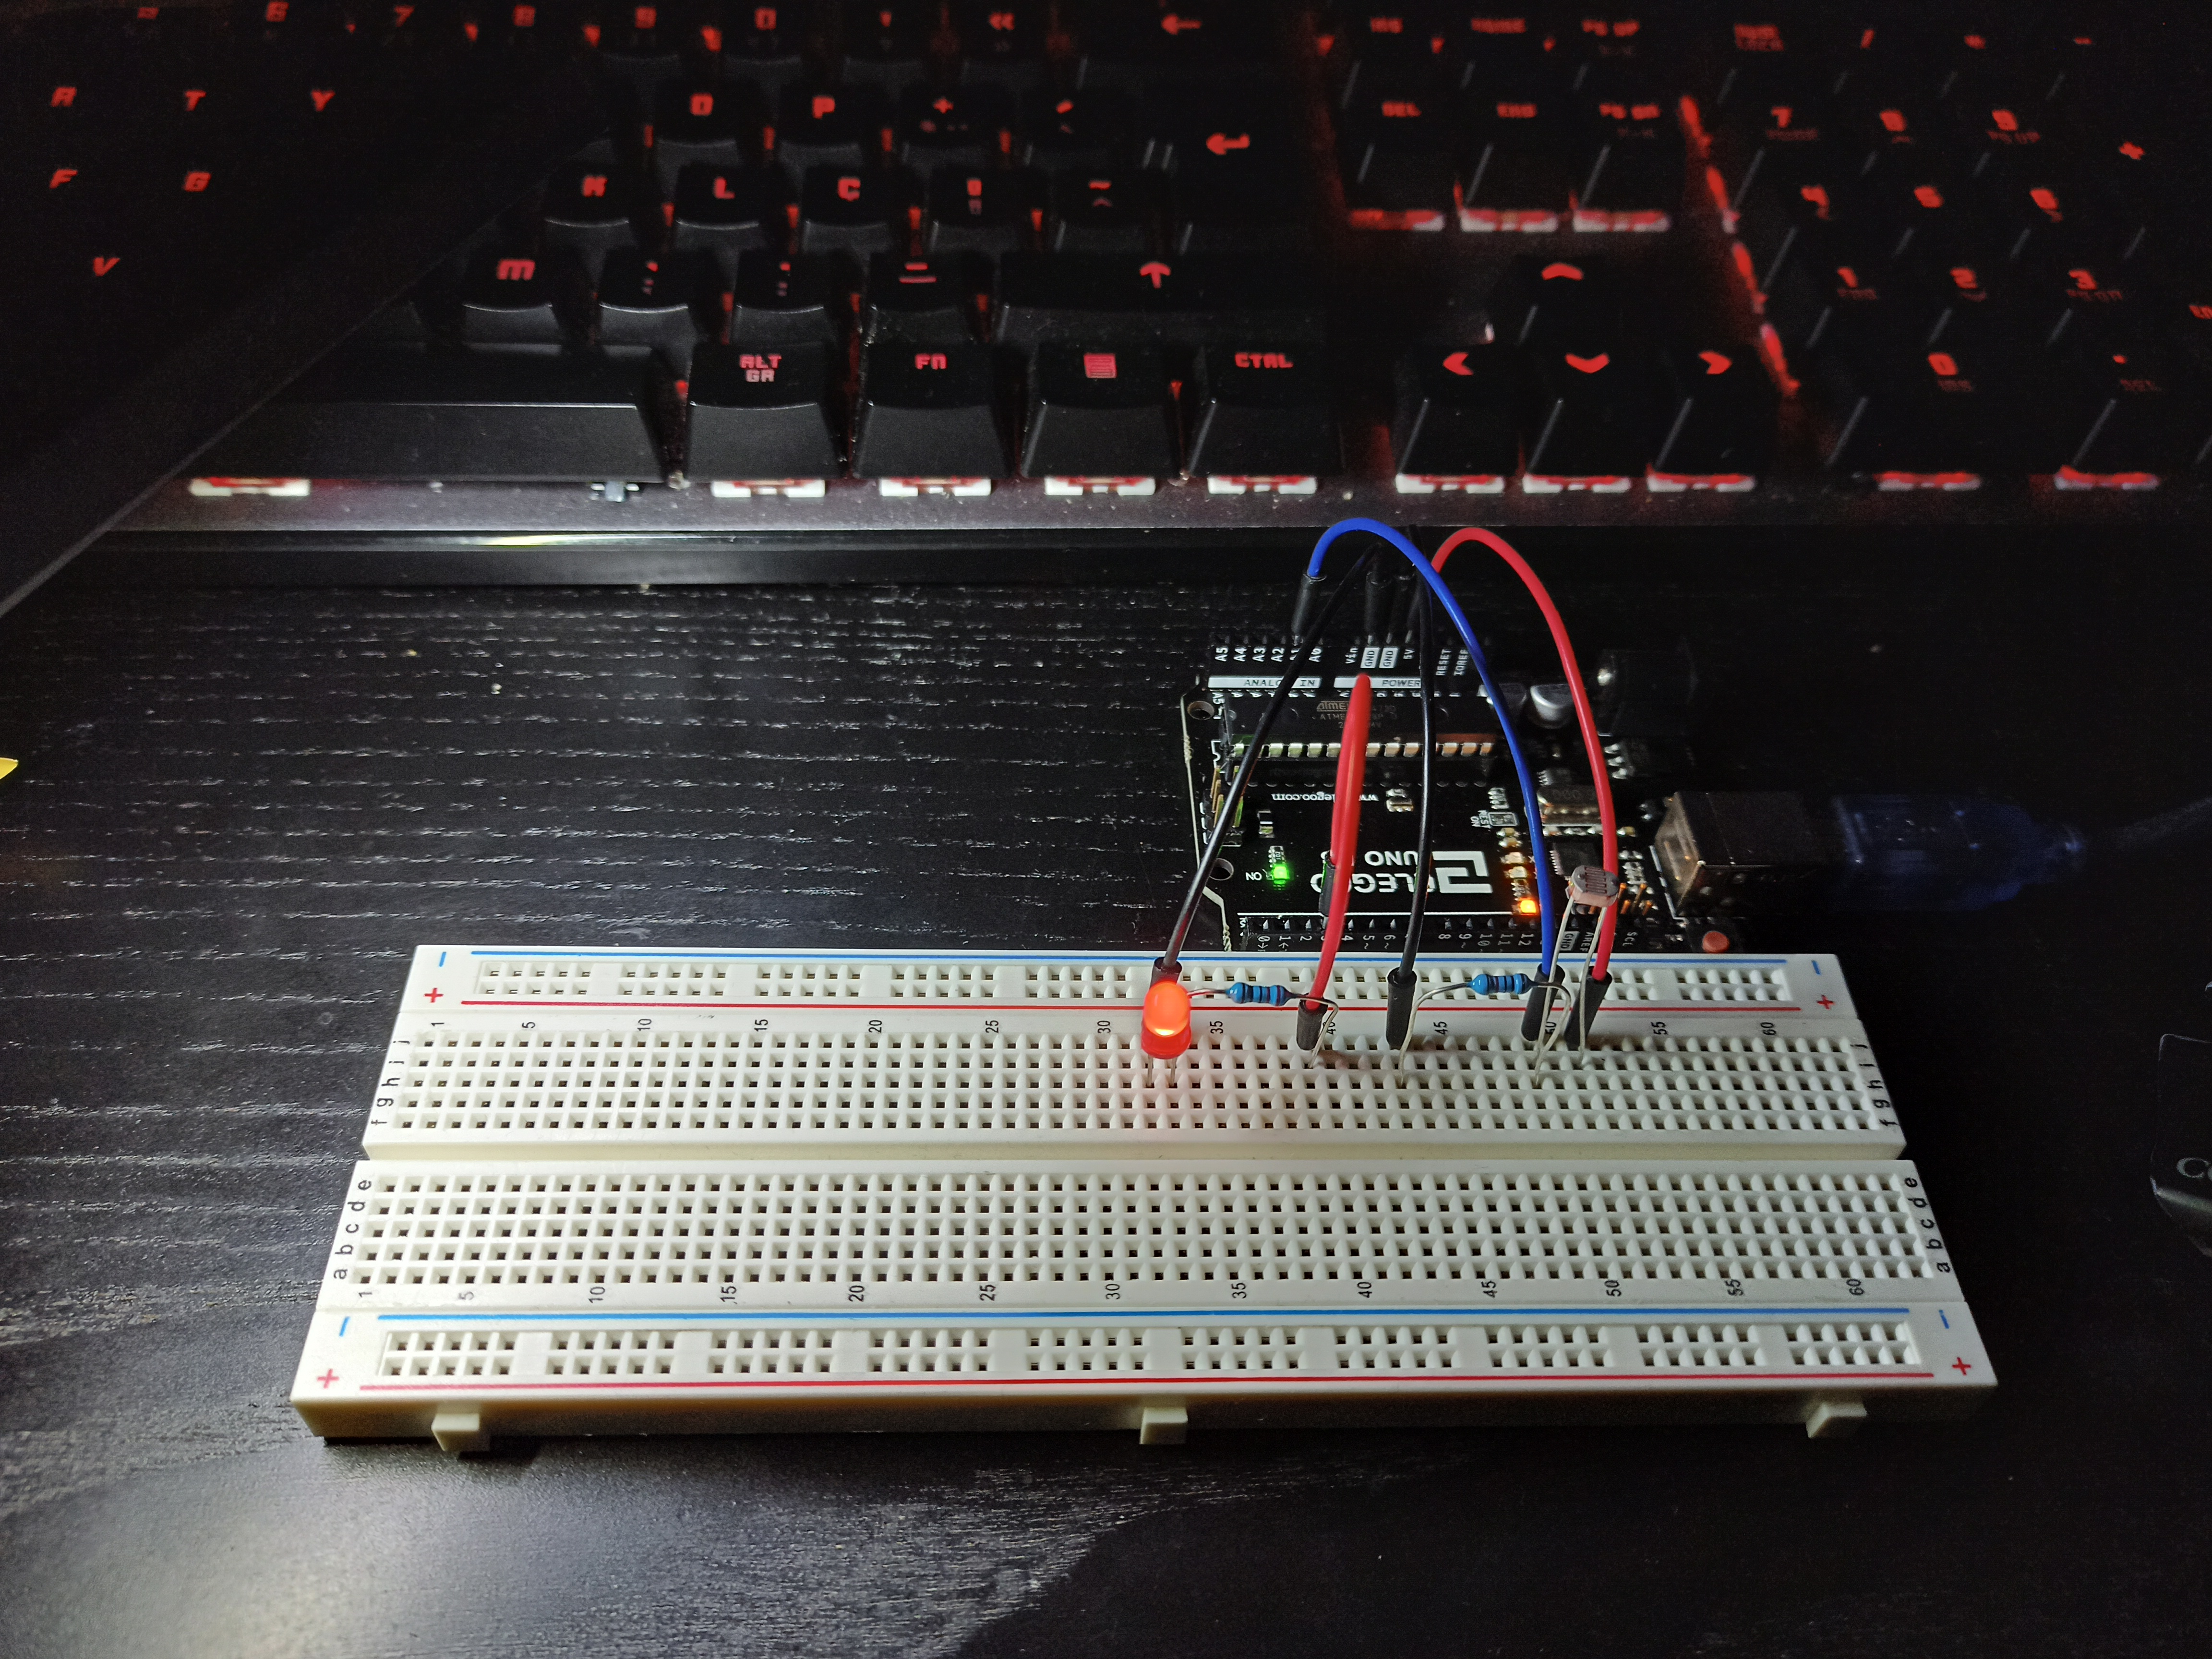
\includegraphics[scale=0.03]{images/testes/sisA_2.jpg}
    \selectlanguage{portuguese}\caption{LED ligado no nivel 2}
\end{figure}

Com um nível de luz entre luz superior a 800 o LED encontra-se ligado com a potência máxima disponível.

\begin{figure}[H]
    \centering
    \includegraphics[scale=1.1]{images/testes/sisA_SerialMonitor3_original.png}
    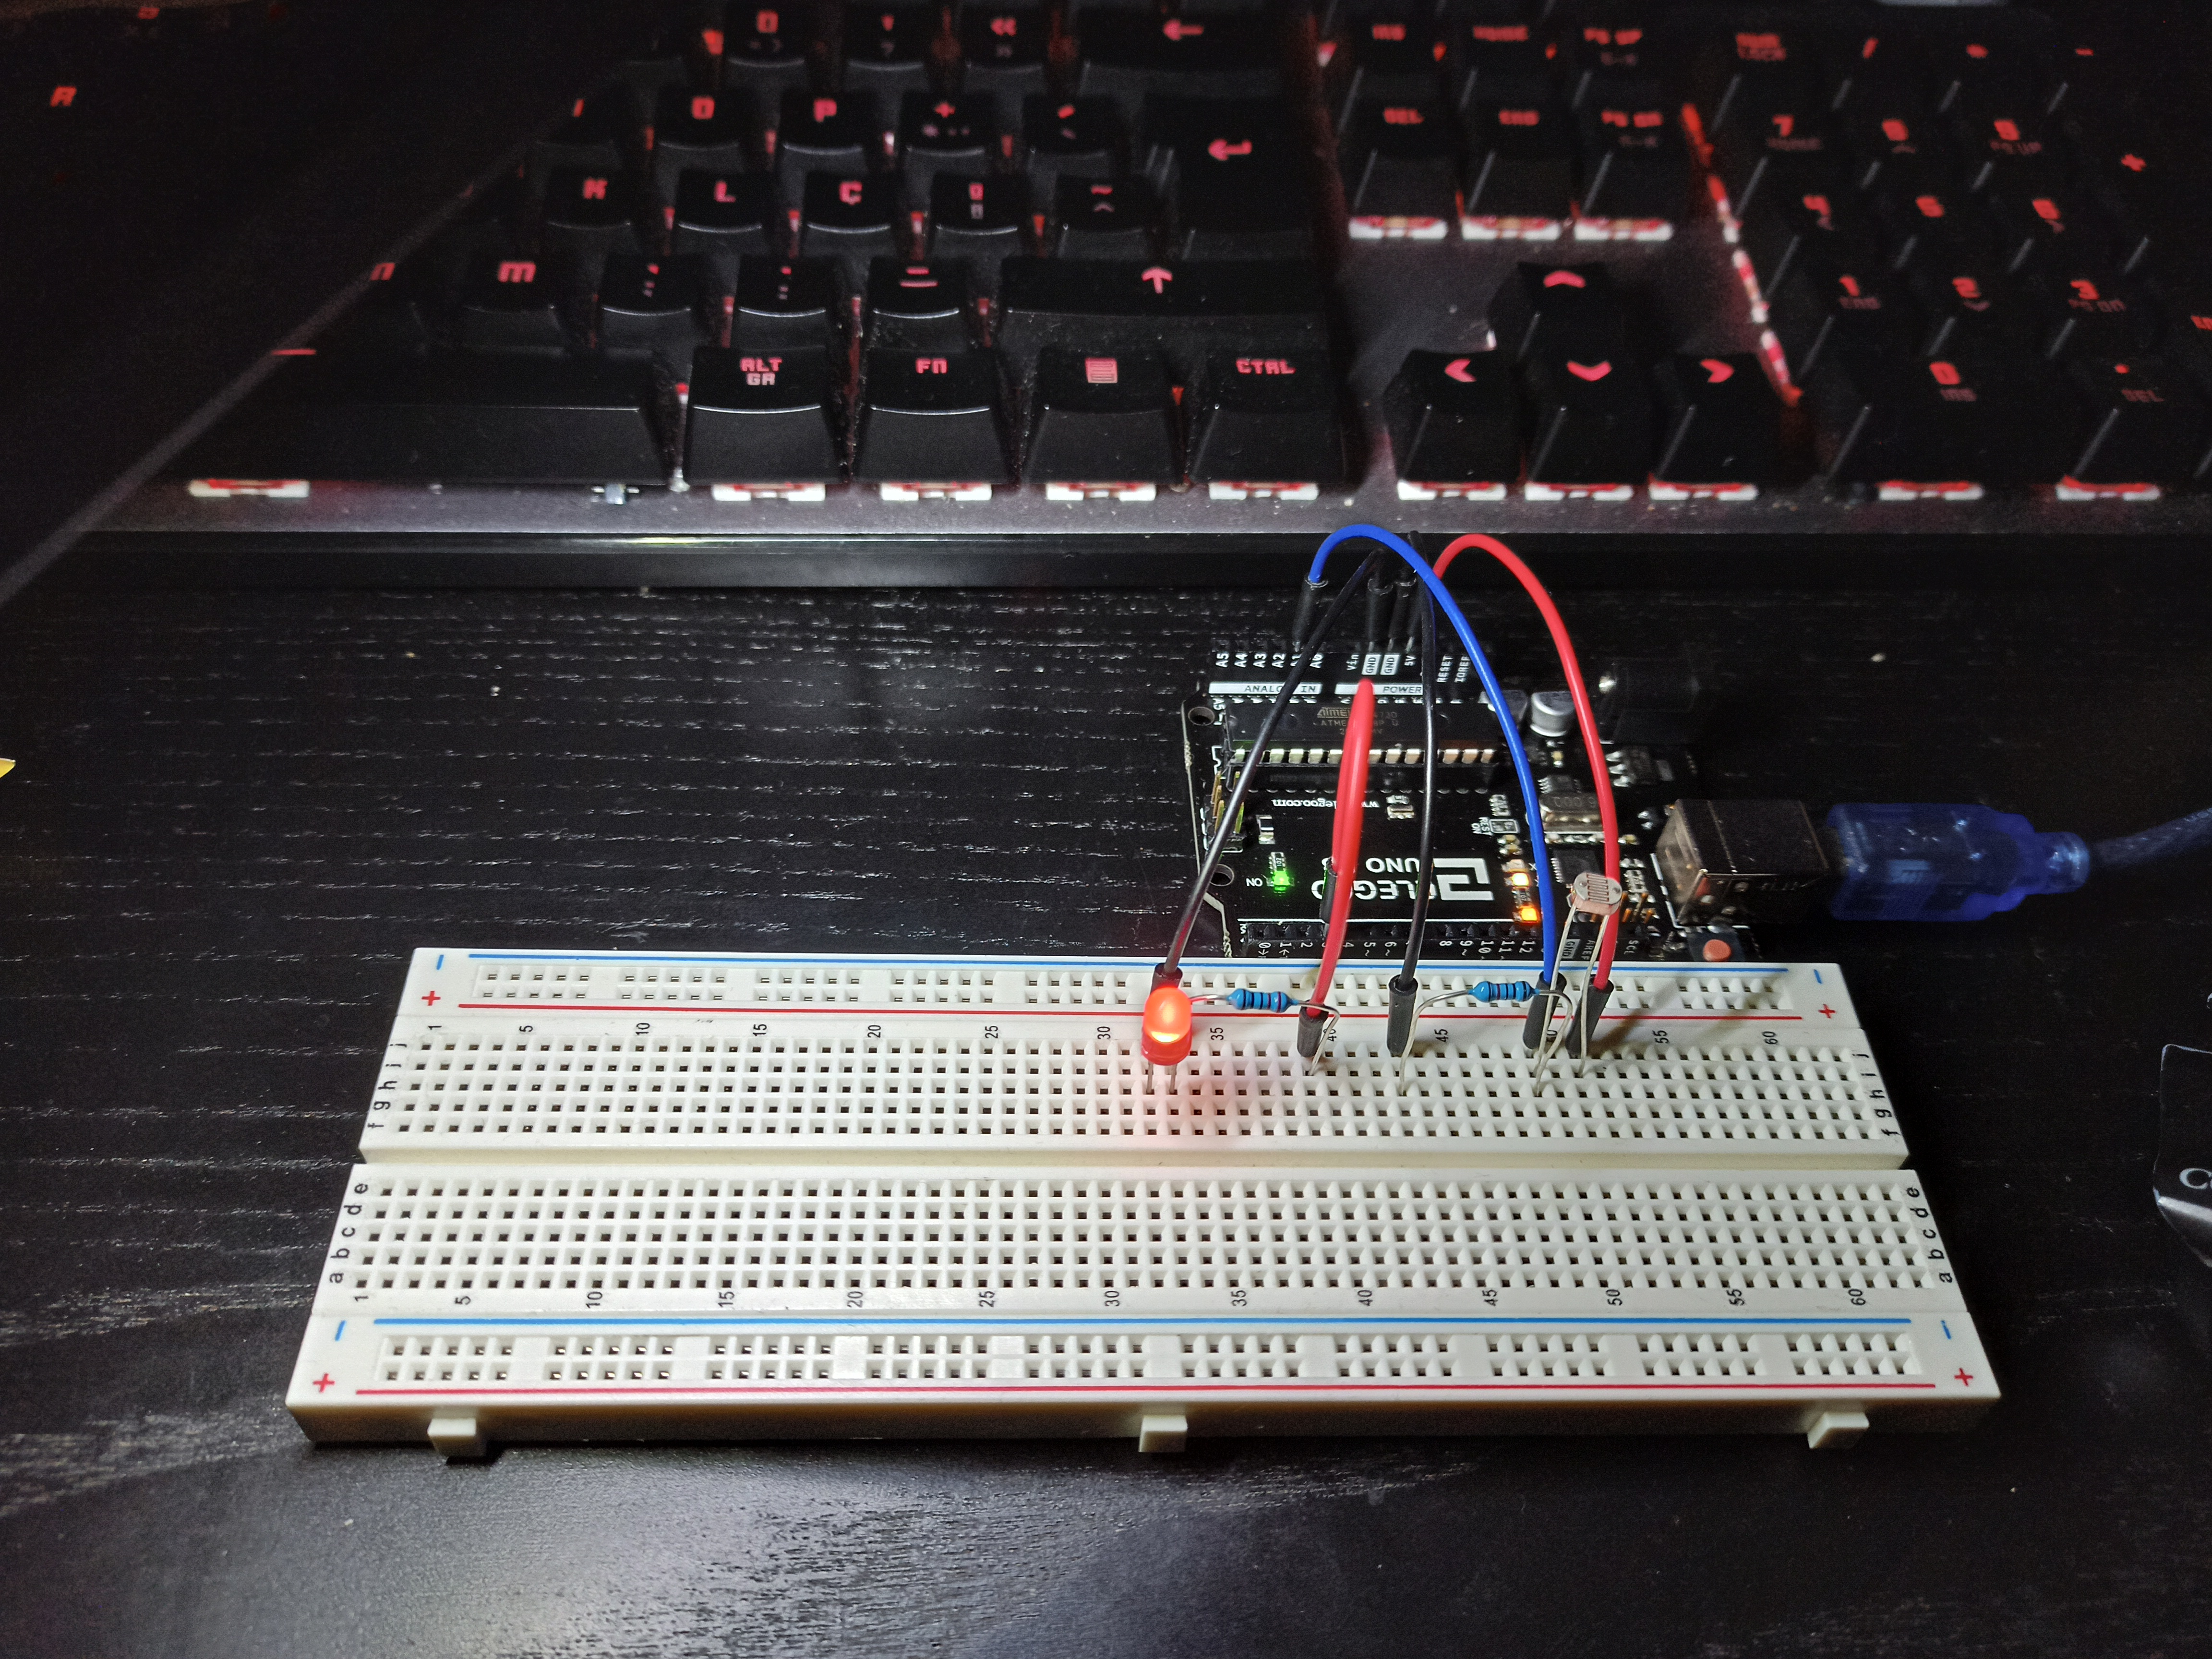
\includegraphics[scale=0.03]{images/testes/sisA_3.jpg}
    \selectlanguage{portuguese}\caption{LED ligado no nivel máximo}
\end{figure}
    \section{Sistema B – Controlo de Climatização}

Para facilidade de teste, o intervalo de temperaturas é ajustado consoante necessário.\\

\begin{figure}[H]
    \centering
    \includegraphics{images/testes/sisB_serialmonitor.png}
    \selectlanguage{portuguese}\caption{Serial Monitor}
\end{figure}
\textbf{Temperature is to high. Cooling Down.}\\
Temperatura ultrapassou máximo definido.\\
\textbf{Temperature stabilized.}\\
Temperatura alcançou mínimo definido.

\begin{figure}[H]
    \centering
    \includegraphics[scale=0.05,angle=-90]{images/testes/sisB_on.jpg}
    \includegraphics[scale=0.05,angle=-90]{images/testes/sisB_off.jpg}
    \selectlanguage{portuguese}\caption{Stabilized vs Cooling Down}
\end{figure}

    \section{Sistema C – Sistema Acesso ao Estacionamento}


Quando é pressionado o botão "seta para cima" no comando, o servo faz com que o portão abra.

\begin{figure}[H]
    \centering
    \includegraphics[scale=0.03]{images/testes/sisC_Open.jpg}
    \includegraphics[scale=0.0225]{images/testes/ControllerUp.jpg}
    \selectlanguage{portuguese}\caption{Portão Aberto}
\end{figure}


Quando é pressionado o botão "vermelho" no comando, o servo suspende o seu movimento.

\begin{figure}[H]
    \centering
    
    \includegraphics[scale=0.03]{images/testes/sisC_semiOpen.jpg}
    \includegraphics[scale=0.0225]{images/testes/controllerOff.jpg}
    \selectlanguage{portuguese}\caption{Portão Semi-aberto}
\end{figure}


Quando é pressionado o botão "seta para baixo" no comando, o servo faz com que o portão feche.

\begin{figure}[H]
    \centering
    
    \includegraphics[scale=0.03]{images/testes/sisC_Closed.jpg}
    \includegraphics[scale=0.0225]{images/testes/ControllerDown.jpg}
    \selectlanguage{portuguese}\caption{Portão Fechado}
\end{figure}


Foi verificado durante os testes que o sensor de infravermelhos nem sempre deteta os valores corretos do comando. Isto pode ser devido a interferências na corrente, pois a falha na deteção dos códigos é acentuada quando o servo se encontra em movimento.
    \section{Sistema D – Sistema de Segurança}

Quando o sensor PIR deteta movimento fica `suspenso' durante um certo tempo em que não deteta qual movimento. Terminando este intervalo, o sensor está `ativo' novamente pelo que pode ocorrer uma repetição da sinalização de `Alarm On', caso o alarme não seja desarmado nesse meio tempo. No entanto, isto não acontece - como pode verificar no vídeo em anexo - é feita uma verificação para caso o alarme já esteja ativo.

Também é verdade para o desarme do alarme com o pressionar do botão. Múltiplos pressionares não desarmam múltiplas vezes o alarme.

\begin{figure}[H]
    \centering
    \includegraphics{images/testes/sisD_serialmonitor.png}
    \selectlanguage{portuguese}\caption{Serial Monitor}
\end{figure}

\begin{figure}[H]
    \centering
    \includegraphics[scale=0.05,angle=-90]{images/testes/sisD_on.jpg}
    \includegraphics[scale=0.05,angle=-90]{images/testes/sisD_off.jpg}
    \selectlanguage{portuguese}\caption{On vs Off}
\end{figure}
    
    \chapter{Performance de Programa - Path}

Para realizar a avaliação em questão foram construídas duas configurações do Sistema de Climatização.

\begin{figure}[H]
    \centering
    \includegraphics[scale=0.6]{images/path.png}
    \selectlanguage{portuguese}\caption{Melhor Path}
    \label{fig:my_label}
\end{figure}

\begin{table}[H]
    \centering
    \begin{tabular}{|c|c|c|}
        \hline
        \multicolumn{1}{|c|}{Temp.} & 
        \multicolumn{1}{|c|}{Fan} & 
        \multicolumn{1}{|c|}{Path}\\
        \hline
        > MAX & LOW & \makecell{T1 = True \\ L1 = False \& L2 = True}\\
        \hline
        > MAX & HIGH & \makecell{T1 = False \& T2 = False \\ L1 = False \& L2 = True}\\
        \hline
        > MIN \&\& < MAX & LOW & \makecell{T1 = False \& T2 = False \\ L1 = True}\\
        \hline
        > MIN \&\& < MAX & HIGH & \makecell{T1 = False \& T2 = False \\ L1 = False \& L2 = True}\\
        \hline
        < MIN & LOW & \makecell{T1 = False \& T2 = False \\ L1 = True}\\
        \hline
        < MIN & HIGH & \makecell{T1 = False \& T2 = True \\ L1 = True}\\
        \hline
    \end{tabular}
    % \caption{Caption}
    % \label{tab:my_label}
\end{table}

\begin{figure}[H]
    \centering
    \includegraphics[scale=0.7]{images/path_worst.png}
    \selectlanguage{portuguese}\caption{Pior Path}
    \label{fig:my_label}
\end{figure}

\begin{table}[H]
    \centering
    \begin{tabular}{|c|c|c|}
        \hline
        \multicolumn{1}{|c|}{Temp.} & 
        \multicolumn{1}{|c|}{Fan} & 
        \multicolumn{1}{|c|}{Path}\\
        \hline
        > MAX & LOW & \makecell{T1 = True \& T2 = False\\ L1 = False \& L2 = True}\\
        \hline
        > MAX & HIGH & \makecell{T1 = False \& T2 = False \\ L1 = False \& L2 = True}\\
        \hline
        > MIN \&\& < MAX & LOW & \makecell{T1 = False \& T2 = False \\ L1 = True \& L2 = False}\\
        \hline
        > MIN \&\& < MAX & HIGH & \makecell{T1 = False \& T2 = False \\ L1 = False \& L2 = True}\\
        \hline
        < MIN & LOW & \makecell{T1 = False \& T2 = False \\ L1 = True \& L2 = False}\\
        \hline
        < MIN & HIGH & \makecell{T1 = False \& T2 = True \\ L1 = True \& L2 = False}\\
        \hline
    \end{tabular}
    % \caption{Caption}
    % \label{tab:my_label}
\end{table}

\newpage

\begin{table}[H]
    \centering
    \begin{tabular}{|c|c|c|}
        \hline
        \multicolumn{1}{|c|}{Estado} & \multicolumn{1}{|c|}{Melhor} & \multicolumn{1}{|c|}{Pior}\\ [0.8ex] 
        \hline
        Superior a Máximo               & 280 µs & 300 µs \\
        \hline
        Estável entre Intervalo         & 20 µs & 20 µs \\
        \hline
        Arrefecimento Entre Intervalo   & 20 µs & 20 µs \\
        \hline
        Inferior a Mínimo Arrefecimento & 200 µs & 220 µs \\
        \hline
        Estável Inferior a Mínimo       & 20 µs & 20µs \\
        \hline
    \end{tabular}
    \selectlanguage{portuguese}\caption{Timer}
\end{table}

Apesar de reduzido, é possível verificar uma diferença no desempenho.
    \section*{Conclusão}
Dados abandonados de nada servem para uma empresa. É apenas com o devido tratamento e análise correta dos dados que uma empresa pode ter qualquer tipo de vantagem que possibilite o sucesso no mercado.

Acreditamos ter cumprido com todos os objetivos definidos.
No que toca à junção de serviços adicionais, tivemos sucesso no tratamento e importação destes mas nem tanto na utilização dos dados.

Conseguimos fazer uso quando colocamos a coluna \textit{populacao\_total[2020]} num campo `Legend' mas em campos tipo `Value' o PowerBi realiza automaticamente `COUNT' das linhas da coluna. Isto era verdade para ambos os dados importados.

Em jeito de conclusão, a utilização de dashboards impulsiona por completo a produtividade e facilidade na toma de decisões de qualquer gestor de empresa, e permite uma completa descrição do negócio em questão e do seu estado atual.
\end{document}